% \documentclass[pdftex,10pt,aspectratio=169]{beamer}
\documentclass[handout,pdftex,10pt,aspectratio=169]{beamer}

% Format
\usetheme{Madrid}
\usepackage{beamercolorthemeMIT}

% % Format (Emilia's choice)
% \usetheme{CambridgeUS}
% \setbeamertemplate{items}[ball]
% \setbeamertemplate{navigation symbols}{}
% \setbeamercolor{item projected}{bg=red}
% \useoutertheme{infolines}
% \setbeamersize{text margin left=8mm}
% \setbeamersize{text margin right=8mm}
% \setbeamercolor{itemize item}{fg=black}
% \setbeamercolor{enumerate item}{fg=black}

% \beamertemplatenavigationsymbolsempty
\setbeamertemplate{headline}{}
\setbeamertemplate{navigation symbols}{}

\usepackage{fancyvrb}
\fvset{fontsize=\footnotesize}
\RecustomVerbatimEnvironment{verbatim}{Verbatim}{}

\usepackage{color}
\usepackage{float}
\usepackage{tikz}
\usetikzlibrary{positioning,shapes.geometric,arrows}
\usetikzlibrary{decorations.markings}

% \usepackage{enumitem}
\usepackage{listings}
\usepackage{verbatim}
\usepackage{amsmath}
\usepackage{caption}
\usepackage{booktabs}
\usepackage{hyperref}
\usepackage{multirow}
%\usepackage{tabularx}
\usepackage[parfill]{parskip} % Don't indent
% \usepackage{setspace}
\usepackage{graphicx}
%\usepackage{fancybox, longtable}
\usepackage{amssymb,amsfonts,bm}
\usepackage{wasysym}
\usepackage{xcolor}
\usepackage{colortbl}
% \newcommand\smallfont{\fontsize{7}{7}\selectfont}
\usepackage{dcolumn,booktabs,multirow,rotating}

\newcommand{\backupbegin}{
  \newcounter{finalframe}
  \setcounter{finalframe}{\value{framenumber}}
}
\newcommand{\backupend}{
  \setcounter{framenumber}{\value{finalframe}}
}

% \newcommand\Wider[2][3em]{%
% \makebox[\linewidth][c]{%
%   \begin{minipage}{\dimexpr\textwidth+#1\relax}
%   \raggedright#2
%   \end{minipage}%
%   }%
% }

%Emilia's addition
% \usepackage{sansmathaccent}
% \pdfmapfile{+sansmathaccent.map}

% == New Commands
% = For general typesetting
% \newcommand\spacingset[1]{\renewcommand{\baselinestretch}{#1}\small\normalsize}
\renewcommand\r{\right}
\renewcommand\l{\left}

% = For stats & econometrics
\newcommand{\indep}{\mbox{$\perp\!\!\!\perp$}}
\renewcommand{\epsilon}{\varepsilon}
\newcommand\ud{\mathrm{d}}
\newcommand\dist{\buildrel\rm d\over\sim}
\newcommand\ind{\stackrel{\rm indep.}{\sim}}
\newcommand\iid{\stackrel{\rm i.i.d.}{\sim}}
\newcommand\logit{{\rm logit}}
\newcommand\cA{\mathcal{A}}
\newcommand\cN{\mathcal{N}}
\newcommand\E{\mathbb{E}}
\newcommand\V{\mathbb{V}}
\newcommand\cJ{\mathcal{J}}
\newcommand\y{{\bm y}}
\newcommand\X{{\bm X}}
\newcommand\x{{\bm x}}
\newcommand\eps{{\bm\varepsilon}}
\newcommand\zero{{\bm 0}}
\newcommand\be{{\bm\beta}}
\renewcommand\b{{\bm b}}
\newcommand\C{{\bm C}}
\newcommand\D{{\bm D}}
\newcommand\I{{\bm I}}
\newcommand\Z{{\bm Z}}
\newcommand\eeta{{\bm \eta}}
\DeclareMathOperator*\plim{plim}
\DeclareMathOperator\rank{rank}
\DeclareMathOperator{\sgn}{sgn}
\def\independenT#1#2{\mathrel{\rlap{$#1#2$}\mkern2mu{#1#2}}}
\definecolor{light-gray}{gray}{0.8}

\graphicspath{{fig}}


%% preamble
\title[Git workshop]{Git for Social Scientists: Introduction to Version Control with Git}
\author[Tomoya]{Tomoya Sasaki%
\thanks{This slide deck is heavily inspired by the workshop materials by Suyeol Yun and Shiro Kuriwaki.}}
\institute[MIT]{Massachusetts Institute of Technology}
\date[Fall 2022]{November 4th, 2022}

\begin{document}

%%%%%%%%%%%%%%%%%%%%%%%%%%%%%%%%%%%%%%%%%%%%%%%%%%%%%%%%%%%%%%%%%%%%%%%%%%%%%%%
\begin{frame}{Before we start today...}
  \begin{itemize}
    \item Create a Github account
    \item Share your account name with me at tomoyas@mit.edu
    \item If possible (or necessary), install Git in your computer (check \url{https://happygitwithr.com/install-git.html})
  \end{itemize}
\end{frame}

\begin{frame}
  \titlepage
  \end{frame}


\begin{frame}{Introduction}
  \begin{columns}[c]
    \begin{column}{0.65\linewidth}
      \centering
      \visible<1->{
\includegraphics[width = 0.95\linewidth]{git_companylist.png}
      Companies using Git}
    \end{column}\hfill
    \begin{column}{0.33\linewidth}
      \centering
      \visible<2->{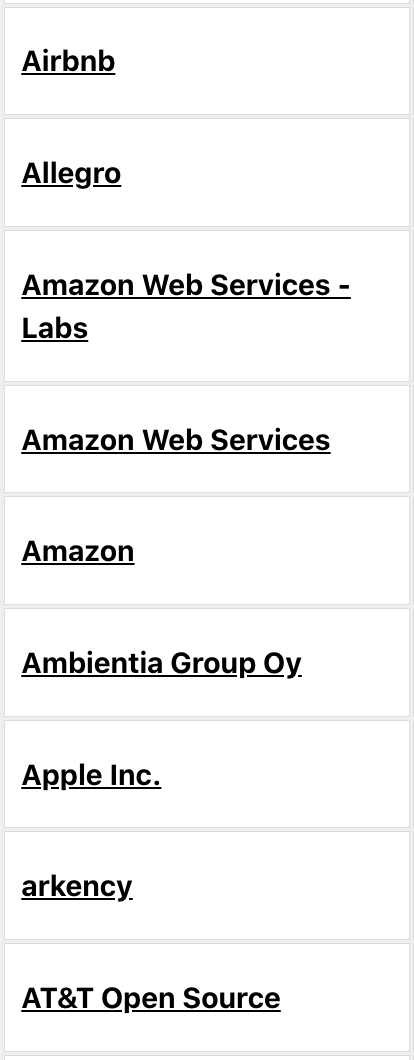
\includegraphics[width = 0.5\linewidth]{github_companylist.png} \\
      Companies using Github}
    \end{column}
  \end{columns}
\end{frame}


\begin{frame}{Introduction}
  \begin{itemize}[<+->]  \setlength\itemsep{-3pt}
    \item Why Git? Why Github? Why version control?
    \item These are essential tools for programmers
    \item How about social social scientists?
    \item My opinion: Social scientists also benefit from version control with Git \vspace{-5pt}
    \begin{itemize} \setlength\itemsep{-5pt}
      \item Increase in collaborative projects
      \item Demand for clean replication materials
      \item Complex data manipulation/preprocessing/analysis
    \end{itemize}
    \item ``Code and Data for the Social Sciences: A Practitioner's Guide''
    by Gentzkow and Shapiro has a chapter dedicated for version control
    \medskip
    \item This workshop \vspace{-5pt}
    \begin{itemize} \setlength\itemsep{-5pt}
      \item Introduction to version control
      \item Pros and cons of Git/Github
      \item Brief introduction to these tools (how Git/Github works and how to use them)
    \end{itemize}
  \end{itemize}
\end{frame}


\begin{frame}{What is version control?}
  \begin{itemize}[<+->]
    \item Version control: tracking and managing changes to file content
    \item Git: (the most popular) software for version control
    \item Github: service to host your git on the Internet
    (alternatives include GitLab, Bitbucket ...)
    \item Repository: unit of a version control project,
    your project folder with a subfolder named \texttt{.git}
    \begin{itemize}
      \item Often simply called ``repo''
      \item \texttt{.git} folder in a repository tracks and stores every single change you make in the corresponding repository
    \end{itemize}
    \medskip
    \item I focus on Git/Github  because they are extremely popular
    than their alternatives
  \end{itemize}
\end{frame}


\begin{frame}{Benefit of Git/Github: Tracking who/how/when}
  \setlength{\leftmarginii}{10pt}
  \begin{columns}%[T]
    \begin{column}{0.46\linewidth}
    \begin{itemize}
      \item<1-> You can identify %\vspace{-5pt}
      \begin{itemize}
        \item<1-> who made changes
        \item<2-> how they made the changes
        \item<3-> when they made the changes
      \end{itemize}
      \item<4-> You can check the entire history since you created a repo
      and move back to previous versions easily (undo changes)
      \item<5-> Github can visualize them nicely
      \medskip
      \item<7-> Useful when you
      \begin{itemize}
        \item<7-> want to revert your (particular) changes
        \item<8-> work on a collaborative project
      \end{itemize}
      \medskip
      \item<9-> You don't need to keep
      \begin{itemize}
        \item<9-> different versions of the same file: \texttt{clean\_data\_1104.R}, \texttt{clean\_data\_1020.R}
        \item<10-> the same file edited by different people: \texttt{clean\_data\_tomoya.R}, \texttt{clean\_data\_adam.R}
      \end{itemize}
    \end{itemize}
  \end{column}\hfill
  \begin{column}{0.53\linewidth}
    \centering
    \visible<5->{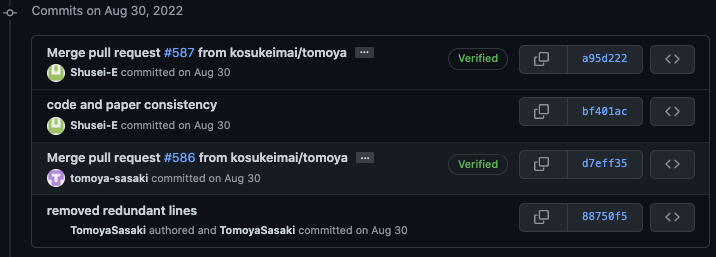
\includegraphics[width = \linewidth]{github_history.png}}
    \visible<6->{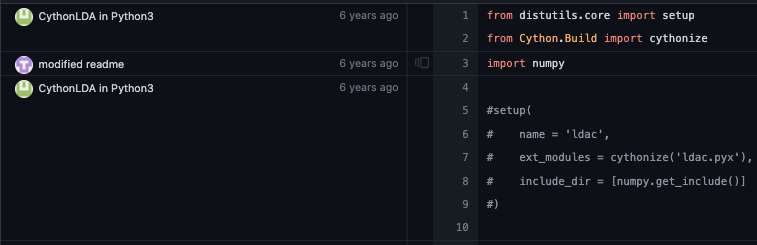
\includegraphics[width = \linewidth]{github_blame.png}}
  \end{column}
  \end{columns}
\end{frame}

\begin{frame}{Benefit of Git/Github: Tracking who/how/when}
  \begin{itemize}[<+->]\setlength\itemsep{-3pt}
    \item You can check how the results change when we try different specification
    \item Easy to track which part of the results changed
  \end{itemize}
  \vspace{10pt}
  \centering
  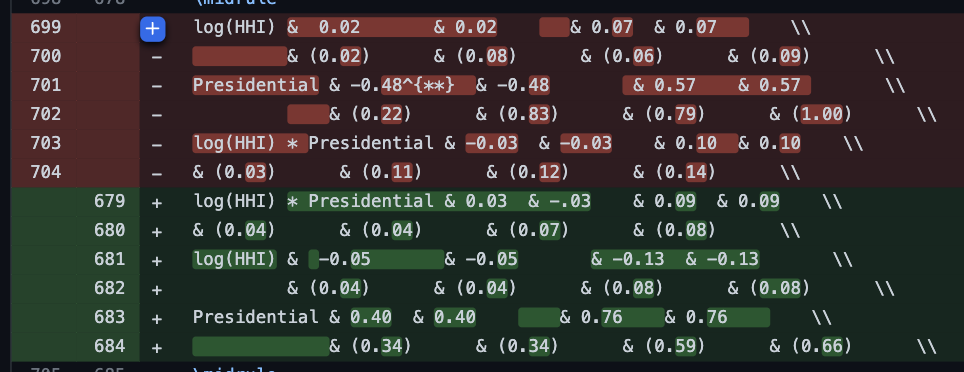
\includegraphics[width = 0.7\linewidth]{github_regression.png}
\end{frame}


\begin{frame}{Other side benefits of Git/Github}
  \begin{columns}[c]
    \begin{column}{0.46\linewidth}
      \begin{itemize}\setlength\itemsep{10pt}
        \item<1-> Hosting a customizable website (free, no ads, tons of templates)
        \item<2-> Contribute to software packages hosting on Github
        \item<3-> Tweak a package developed by someone else for your own purposes
        \item<4-> Send a request to package developer (often happens at ``Issue'')
        \item<5-> Nice integration with popular apps/websites such as RStudio and Overleaf
      \end{itemize}
    \end{column}\hfill
    \begin{column}{0.53\linewidth}
      % \begin{overprint}
      % \centering
      % \onslide<2-3|handout:1>{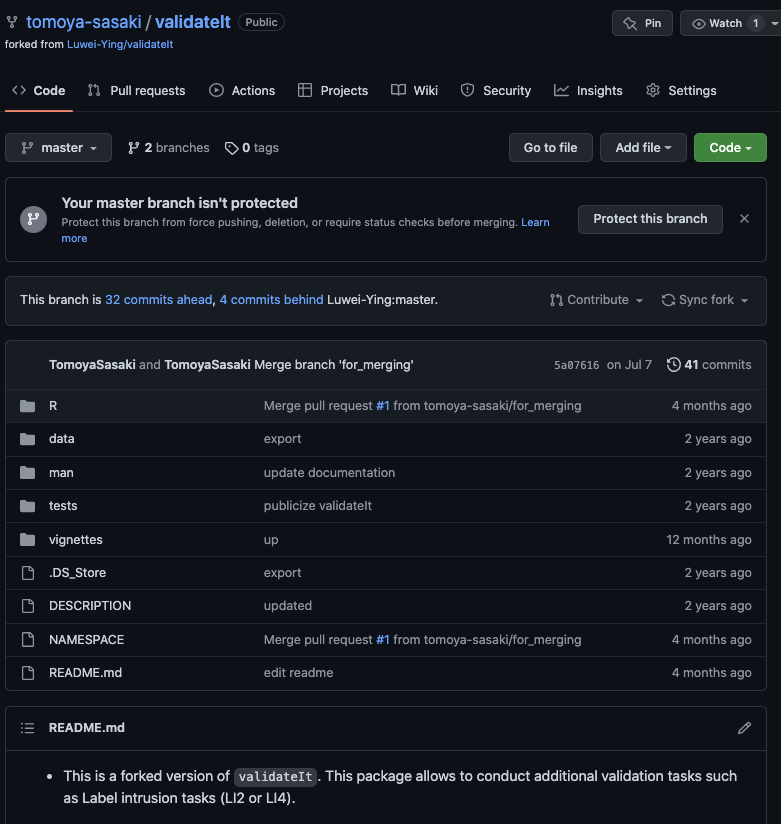
\includegraphics[width = 0.85\linewidth]{github_forked.png}}
      % \onslide<4|handout:2>{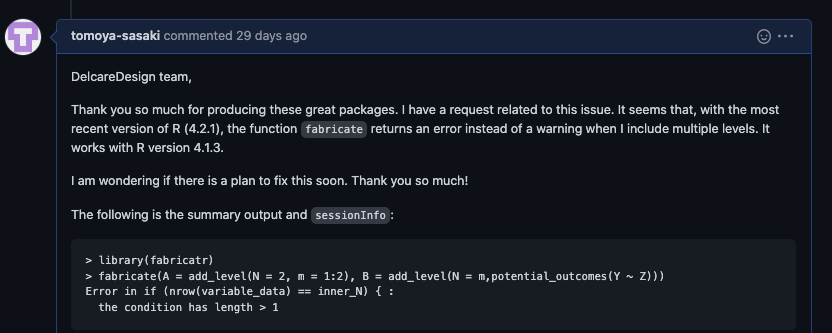
\includegraphics[width = \linewidth]{github_issue.png}}
      % \end{overprint}
      \centering
      \only<1|handout:1>{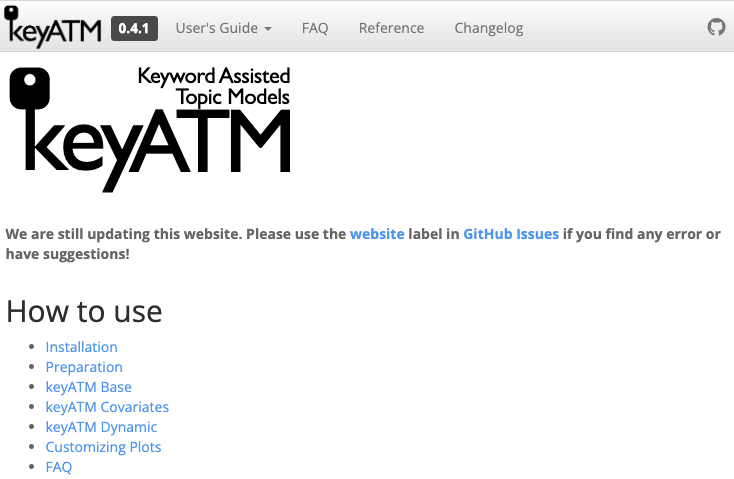
\includegraphics[width = 0.85\linewidth]{github_website.png}}
      \only<2-3|handout:2>{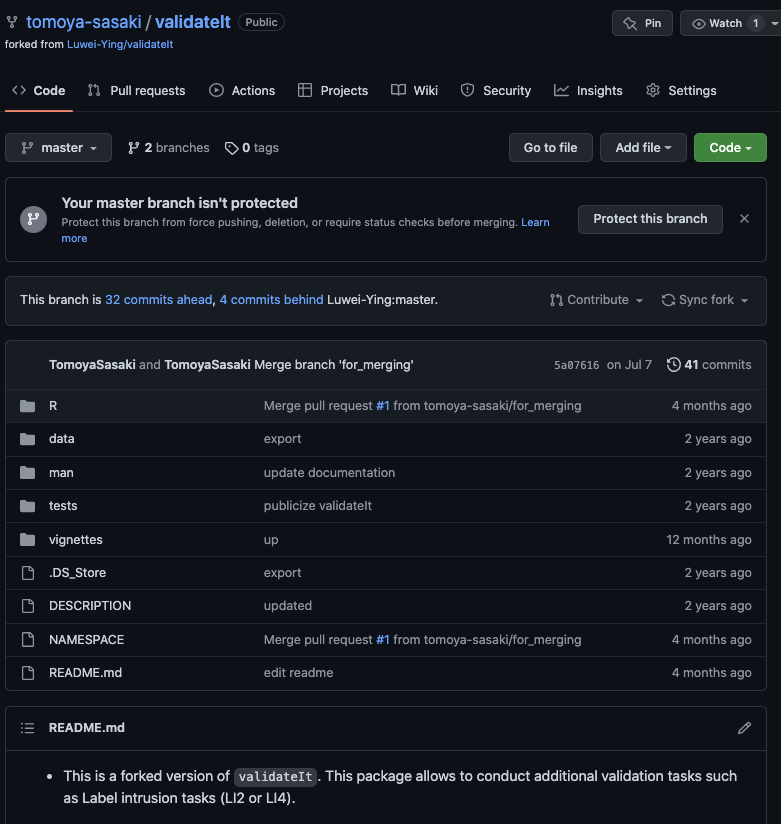
\includegraphics[width = 0.85\linewidth]{github_forked.png}}
      \only<4|handout:3>{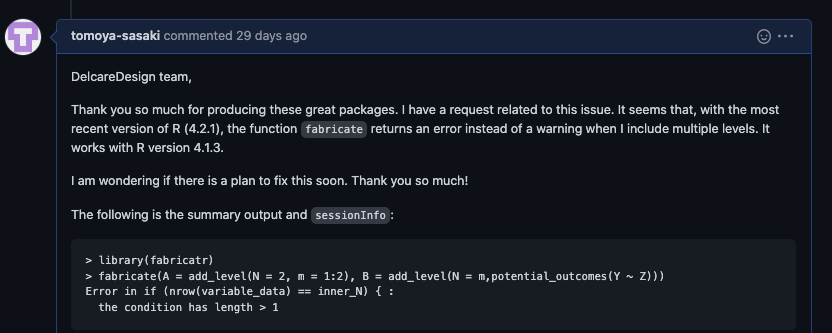
\includegraphics[width = \linewidth]{github_issue.png}}
      \only<5|handout:4>{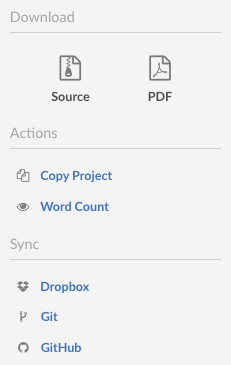
\includegraphics[width = 0.55\linewidth]{github_overleaf.png}}
      \end{column}
  \end{columns}
\end{frame}

\begin{frame}[fragile]{Limitations: not suitable for tracking large files}
  \begin{itemize}[<+->]
    \item Github imposes file size limit:
    \begin{itemize}
      \item 25 MB per file limit
      (you can change this limit up to 100MB by changing setup)
      \item 1GB per repo limit
    \end{itemize}
    \item Remember that \texttt{.git} tracks and stores all the change you make in a repo
    \item[] $\leadsto$ if you store a huge file in the repo and let \texttt{.git} tracks
    its changes, the \texttt{.git} folder can grow quite huge
    \medskip
    \item Use \texttt{.gitignore} to specify files that Git should not track (``ignore'')
    \begin{Verbatim}[frame=single, label=.gitignore]
      *.csv # ignore csv files
      /data/ # ignore any file in data folder
    \end{Verbatim}
    \item Include huge files as well as sensitive files that contain password, API key etc in \texttt{.gitignore}
  \end{itemize}
\end{frame}


\begin{frame}[fragile]{Limitations: not great if you want to track non-text files}
  \begin{columns}[c]
    \begin{column}{0.46\linewidth}
      \begin{itemize}[<+->]\setlength\itemsep{10pt}
        \item Git cannot track line by line changes for non-text files such as
        PDF, Microsoft Word/Excel/Powerpoint, JPG, ...
        \item Note that Git still tracks changes
        \item The value of Git/Github is limited
        \medskip
        \item In the right example, Git/Github recognizes the changes as the changes in file sizes\\
        $\leadsto$ even though you update a figure in PDF or PNG format,
        Git/Github might not recognize it unless the file size changes...
      \end{itemize}
    \end{column} \hfill
    \begin{column}{0.53\linewidth}
      \centering
      \only<4->{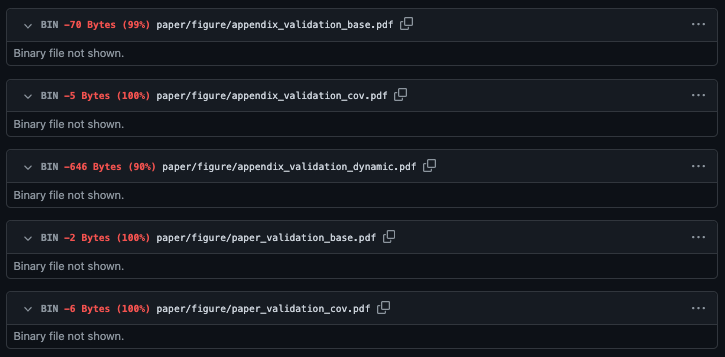
\includegraphics[width = \linewidth]{github_pdf.png}}
    \end{column}
  \end{columns}
\end{frame}


\begin{frame}{How Git tracks files}
  \begin{columns}[c]
    \begin{column}{0.46\linewidth}
      \begin{itemize}[<+->] \setlength\itemsep{10pt}
        \item Git tracks changes in files with ``\textbf{commit}''
        \item Changes between commits are called ``\textbf{diff}''
        \item Each commit is a snapshot of your repo at specific times
        \item Commit has a human-readable message and an (first few characters of) commit ID
        \item Commit is not automatic and you actively make a ``commit'' with a message
        \item Ideally commit should be atomic units of change that represent a specific idea
        \item You need to ``\textbf{stage}'' the files you want to add to commit (more later)
      \end{itemize}
    \end{column} \hfill
    \begin{column}{0.53\linewidth}
      \centering
      \only<1->{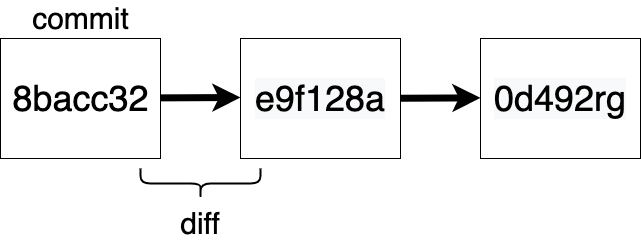
\includegraphics[width = \linewidth]{github_commit.png}}
      \begin{itemize}
        \item<4-> 8bacc332: ``test commit''
        \item<4-> e9f128a: ``edit analysis code''
        \item<4-> 0d492rg: ``add new analysis''
      \end{itemize}
    \end{column}
  \end{columns}
\end{frame}


\begin{frame}{Github and more on repos}
  \begin{itemize}[<+->]%\setlength\itemsep{10pt}
    % \item Commit is a Git feature
    \item If you just work on your local repos (and only on one computer), you don't need Github
    \item Repos: unit of a version control project,
    contains a folder with a subfolder named \texttt{.git}
    \begin{itemize}
      \item Local repos: repos (folder) in your own computer, ordinary project folder with subfolder named \texttt{.git}
      \item Remote repos: repos (folder) in a web hosting services such as Github
    \end{itemize}
    \item Remote repos such as Github...
    \begin{itemize}
      \item come with unique URL (\texttt{https://github.com/username/reponame.git})
      \item are basically a copy of your local repos
      \item nicely visualize your commits
      and also serve as a backup of your codes (remember, not for data)
      \item useful when you work on the same project with multiple computers
    \end{itemize}
    \item You can choose remote repo to be public or private
    \item Github accounts let you create unlimited number of private repos
    with upto 3 collaborators unlimited number of public repos with unlimited number of collaborators
  \end{itemize}
\end{frame}


\begin{frame}{How to interact with remote repos on Github}
  \begin{columns}[c]
    \begin{column}{0.6\linewidth}
      \begin{itemize}\setlength\itemsep{10pt}
        \item<1-> Interaction with remote repos: \textbf{pull} and \textbf{push}
        \item<2-> You \textbf{push} the commits you made to remote repos
        \item<3-> You \textbf{pull} new commits on remote repos
        \item<3-> Technically ``pull'' does \textbf{fetch} and \textbf{merge}
      \end{itemize}
    \end{column} \hfill
    \begin{column}{0.39\linewidth}
      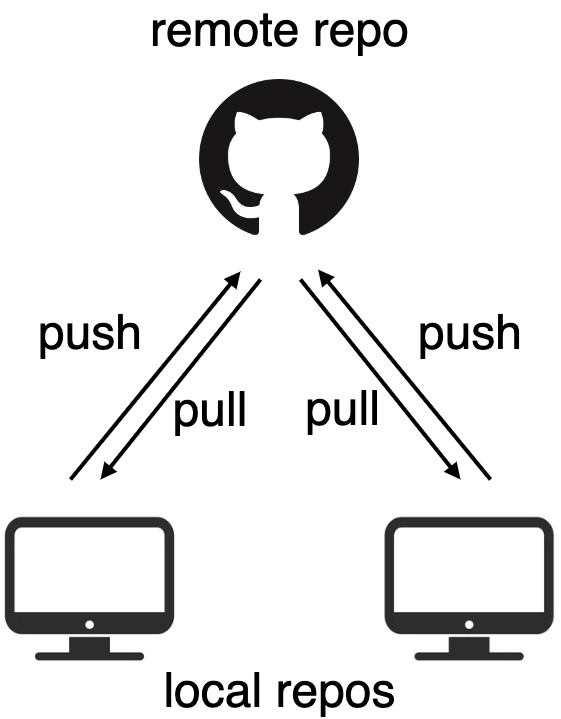
\includegraphics[width = 0.9\linewidth]{github_pullpush.png}
    \end{column}
  \end{columns}
\end{frame}


\begin{frame}{How to use Git/Github}
  \begin{itemize}[<+->]
    \item So far, we have covered some fundamental concepts around Git/Github
    \item But how do we initialize a repo and commit/pull/push in practice?
    \item Command line, Github desktop app etc
    \item This workshop focuses on RStudio
    \item I personally use command line
  \end{itemize}
\end{frame}


\begin{frame}{General (suggestive) initialization}
  \begin{enumerate}[<+->]
    \item Establish a connection between your computer and Github
    \item Create a repo on Github (create a public one for now)
    \item \textbf{Clone} your remote repo on Github to your computer (can be any location).
    This is your local repo.
    \item Edit \texttt{.gitignore} to make sure that Git won't track any sensitive or huge file
  \end{enumerate}
  \medskip
  \begin{itemize}[<+->]
    \item If you have any existing project that you want to track with Git, create a remote repo
    on Github, clone it to your computer (i.e., local repo), and move codes and folders into the local repo
  \end{itemize}
\end{frame}


\begin{frame}{General (suggestive) daily workflow}
    \begin{enumerate}[<+->]
    \item Edit, add, or delete files in your repo
    \item Stage files you want to add to commit and
    make a commit when you make some changes that represent a specific idea or solve particular issues
    \begin{itemize}
      \item Add lines to clean data
      \item Add lines to visualize regression results
      \item Delete lines that are irrelevant anymore
    \end{itemize}
    \item Push when you make a set of commits or when you call it a day
    \item Pull any new commits in the remote repo if there are commits and pushes to the remote repo
    from other computers
    \item Repeat the process above
  \end{enumerate}
  \medskip
  \begin{itemize}[<+->]
    \item Push at least once a day if you make any edit
    \item Let's try out with Github and RStudio
  \end{itemize}
\end{frame}


\begin{frame}{Setup authentication}
  \begin{itemize}[<+->]
    \item When we interact with a remote Git server,
    such as GitHub, we need to provide credentials
    \item Github provides two authentication methods, HTTPS and SSH
    \item I recommend HTTPS and will use HTTPS in this workshop
    \item Procedure
    \begin{enumerate}
      \item Go to  \url{https://github.com/settings/tokens} and click ``Generate token''
      \item Decide the scope. Choose (at least) ``repo'', ``user'', and ``workflow''.
      \item Click ``Generate token''. This is the same as the password to interact  with Git. You shouldn't show this to anyone.
      \item Copy the generated strings (PAT, personal access token)
      \item Open RStudio and run \texttt{gitcreds::gitcreds\_set()}
      (Install the \texttt{gitcreds} package beforehand)
      \item Paste your PAT
      \item RStudio stores and remembers PAT for you
    \end{enumerate}
  \end{itemize}
\end{frame}

\begin{frame}{How Git/Github handle collarborative projects}
  \begin{columns}[c]
    \begin{column}{0.55\linewidth}
      \begin{itemize}[<+->]\setlength\itemsep{10pt}
        \item Easy collaboration is a distinct feature of Git
        \item Key concepts: \textbf{branch} and \textbf{fork}
        \item Branches are parallel universe of a repo
        \item Main branch is the default branch and should contain stable version
        \item You contribute to a repo by creating a new branch in isolation from changes
        that other people are making to the repo
        \item Whenever you work on a collaborative project, you should always create a new branch
      \end{itemize}
    \end{column} \hfill
    \begin{column}{0.44\linewidth}
      \only<7->{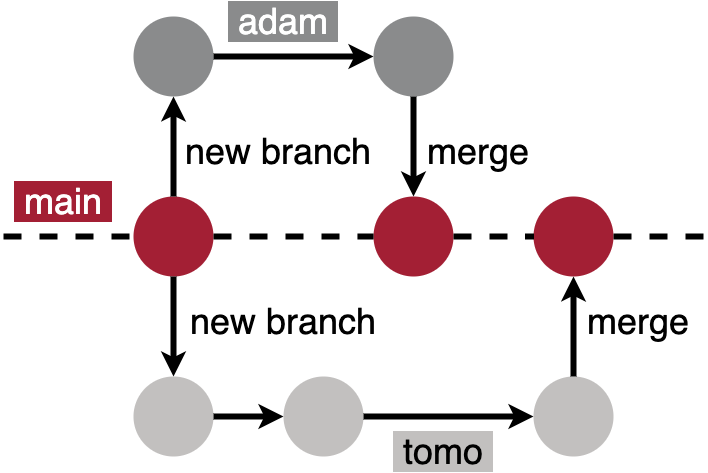
\includegraphics[width = \linewidth]{github_branch.png}}
      \begin{itemize}
        \item<7-> Each circle represents ``commit''
        \item<8-> In this example, Adam and Tomo work on the same project and
        each of them creates a branch
      \end{itemize}
    \end{column}
  \end{columns}
\end{frame}


\begin{frame}{How Git/Github handle collarborative projects}
  \begin{columns}[c]
    \begin{column}{0.55\linewidth}
      \begin{itemize}[<+->] \setlength\itemsep{10pt}
        \item Once your work is done, open \textbf{pull request}, and \textbf{merge} your branch
        into the default branch
        \item Pull request is an opportunity to discuss or check (\textbf{review})
        if the changes you make in your branch won't break the default branch
        \item By merging your branch into the default branch, any edit you make in your branch
        will be reflected in the default branch
        \item When both of them finish their work, they open a pull request and
        merge their branch into the main branch
      \end{itemize}
    \end{column} \hfill
    \begin{column}{0.44\linewidth}
      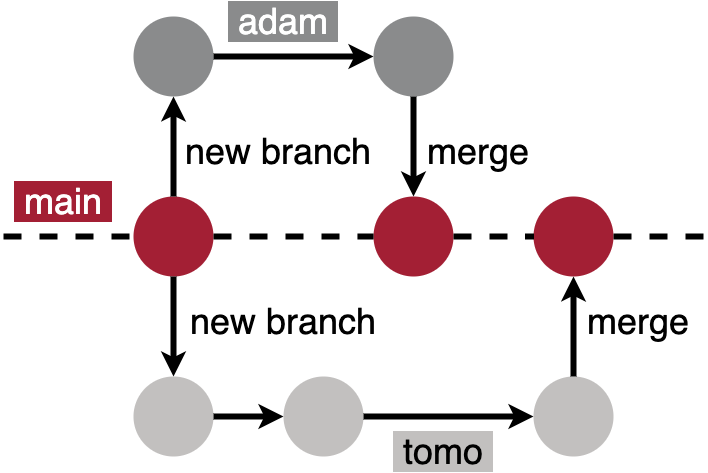
\includegraphics[width = \linewidth]{github_branch.png}
      \begin{itemize}
        \item Each circle represents ``commit''
        \item In this example, Adam and Tomo work on the same project and
        each of them creates a branch
      \end{itemize}
    \end{column}
  \end{columns}
\end{frame}


\begin{frame}{General (suggestive) daily workflow with multiple branches}
  \begin{enumerate}[<+->]
    \item Create a new branch (usually from the default branch)
    \item In your branch...
    \begin{enumerate}
      \item Edit, add, or delete files in your repo
      \item Stage files you want to add to commit and
      make a commit when you make some changes that represent a specific idea or solve particular issues
      \item Push when you make a set of commits or when you call it a day
      \item Repeat the process above
    \end{enumerate}
    \item Create a pull request when you finish your project
    \item Merge your branch into the default branch
  \end{enumerate}
  \begin{itemize}
    \item<10-> Let's try out with Github and RStudio
  \end{itemize}
\end{frame}


\begin{frame}{Working on someone else's repo}
  \begin{columns}[c]
    \begin{column}{0.55\linewidth}
      \begin{itemize}[<+->]\setlength\itemsep{10pt}
        \setlength{\leftmarginii}{10pt}
        \item Even if you have a public repo on Github, only those who have permission
        can directory push and merge to your repo
        \item What to do if you want to contribute to someone else's repo or borrow their idea and
        tailor for your own project?
        \item \textbf{Fork} their project to your Github account
        \begin{itemize}
          \item Original: \texttt{https://github.com/xxx/reponame.git}
          \item Forked repo: \texttt{https://github.com/yourusername/reponame.git}
        \end{itemize}
      \end{itemize}
        \end{column}\hfill
    \begin{column}{0.44\linewidth}
      % \begin{overprint}
      % \centering
      % \onslide<2-3|handout:1>{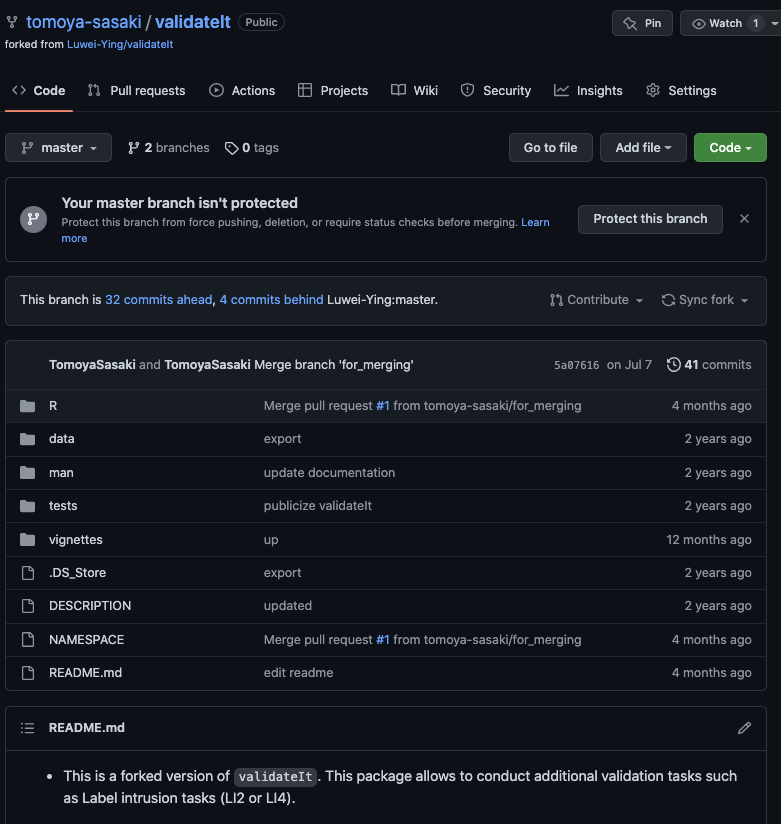
\includegraphics[width = 0.85\linewidth]{github_forked.png}}
      % \onslide<4|handout:2>{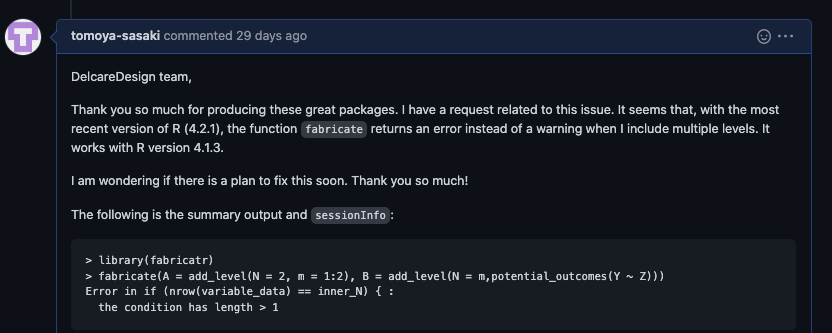
\includegraphics[width = \linewidth]{github_issue.png}}
      % \end{overprint}
      \centering
      \only<4->{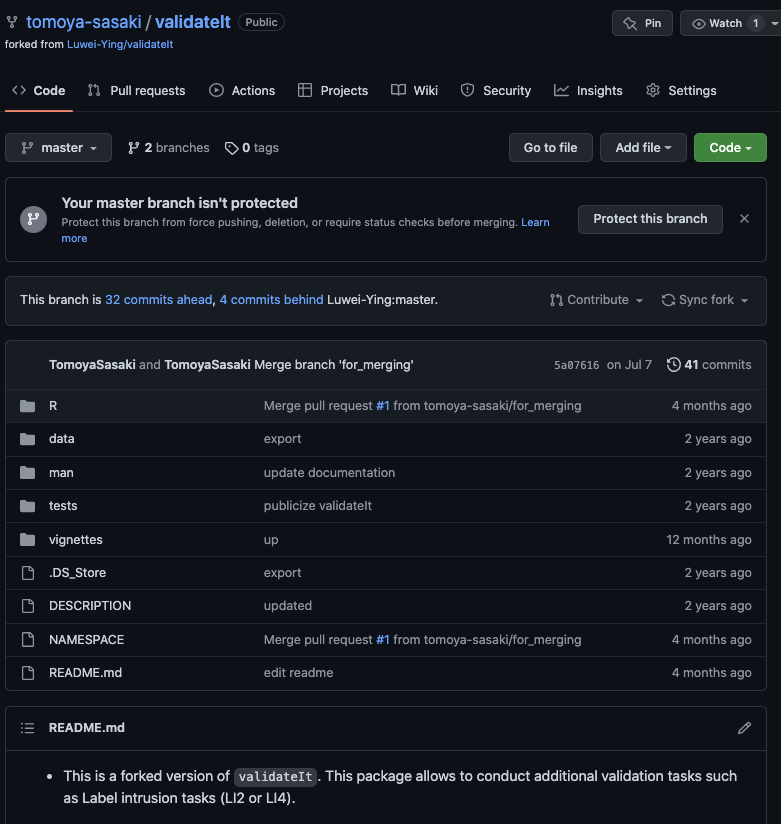
\includegraphics[width = 0.95\linewidth]{github_forked.png}}
      \end{column}
  \end{columns}
\end{frame}


\begin{frame}{Comparison and relationship to alternatives (Dropbox, Google Drive)}
  \begin{itemize}[<+->]
    \item Unlike Dropbox or Google Drive, Git/Github does not automatically track changes
    \item[] $\leadsto$ you need to take (small) action (mostly) when you edit
    \item However, you can make your project folder clean with commits and branches
    \item You can revert your changes easily and flexibly if you make frequent commits
    \item[] $\leadsto$ Dropbox and Google Drive only preserve once-in-a-day snapshots
    \bigskip
    \item Putting Git local repos in Dropbox or Google Drive can be very tricky
    when your Dropbox/Google Drive account is synced to multiple computers
    \item Git does not like autosync (autoupdate) by Dropbox/Google Drive
    \item But you probably want to rely on these other services to store huge data that Git does not track
    \item In my setup, I put Git repos in Dropbox but sync them only with my main computer and
      the same Git repos in my other computers are located in non-Dropbox folders
  \end{itemize}
\end{frame}


\begin{frame}{What's next?}
  \begin{itemize}[<+->]
    \item Working with private repos
    \item (Gradually) Learning how to use git in command lines
    \medskip
    \item Probably you mess up once in a while. I still make mistakes sometimes
    \item You can fix them easily by reverting
  \end{itemize}
\end{frame}


\begin{frame}{Useful resources}
  \begin{itemize}
    \item Happy Git and GitHub for the useR: https://happygitwithr.com/index.html
    \item Git Guide: https://github.com/git-guides
    \item git-vs-dropbox: https://michaelstepner.com/blog/git-vs-dropbox/
  \end{itemize}
\end{frame}


\backupbegin
\backupend
\end{document}
